%versi 2 (8-10-2016)
\chapter{Landasan Teori}
\label{chap:teori}

Pada bab ini dibahas dasar teori yang mendukung berjalannya skripsi ini. Dasar teori yang dibahas yaitu Git, JGit, Selenium WebDriver, dan Apache Commons CLI.

\section{Git}
\label{sec:git} 
Seperti yang telah dijelaskan pada subbab \ref{sec:label}, Git merupakan perangkat lunak \textit{Version Control Systems}. Pada subbab ini, dijelaskan mengenai \textit{Version Control Systems}, cara kerja Git, Git \textit{checkout}, dan operasi-operasi dasar pada Git.   

\subsection{Version Control Systems}
\label{subsec:vcs}
\textit{Version Control Systems} adalah sistem yang merekam perubahan pada \textit{file} atau sekumpulan \textit{file} dari waktu ke waktu\cite{chacon2014pro}.\textit{Version Control Systems} biasanya digunakan  untuk merekam file yang berisi \textit{source code program}, tetapi pada kenyataannya \textit{Version Control Systems} dapat merekam hampir semua jenis file dalam komputer. Terdapat tiga jenis \textit{Version Control Systems}, yaitu: \textit{local Version Control Systems}, \textit{centralized Version Control Systems}, dan \textit{distributed Version Control Systems}.

\subsubsection{Local Version Control Systems}
Metode \textit{version-controlled} yang banyak digunakan orang adalah dengan cara menyalin sekumpulan \textit{file} ke direktori lain\cite{chacon2014pro}. Namun cara tersebut rentan terhadap \textit{error}.
Misalnya, terdapat direktori A dan B, pengguna ingin mengubah \textit{file} yang terdapat pada direktori B, tetapi pengguna lupa kalau dia sedang berada di direktori A, maka pengguna mengubah \textit{file} pada direktori yang salah. Untuk mengatasi masalah tersebut, \textit{programmer} mengembangkan \textit{local Version Control Systems}. 

\begin{figure}[H]
	\centering
		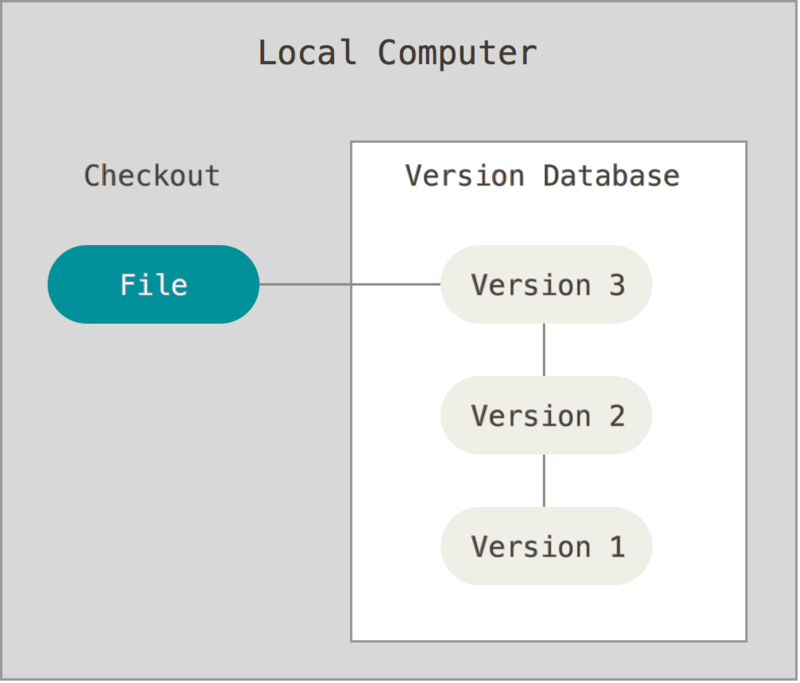
\includegraphics[scale=0.25]{Gambar/localvcs.png}
	\caption{Local version control}
	\label{fig:localvcs}
\end{figure}

Gambar \ref{fig:localvcs} merupakan struktur dari \textit{Local Version Control Systems}. \textit{Database local Version Control Systems} ini tersimpan pada \textit{local} direktori di komputer. \textit{Database} ini menyimpan perubahan \textit{file} ke dalam beberapa versi atau \textit{state}.\textit{Local Version Control}, dapat melakukan \textit{checkout} \textit{file} ke versi atau \textit{state} tertentu.   
 
\subsubsection{Centralized Version Control Systems}
\begin{figure}[H]
	\centering
		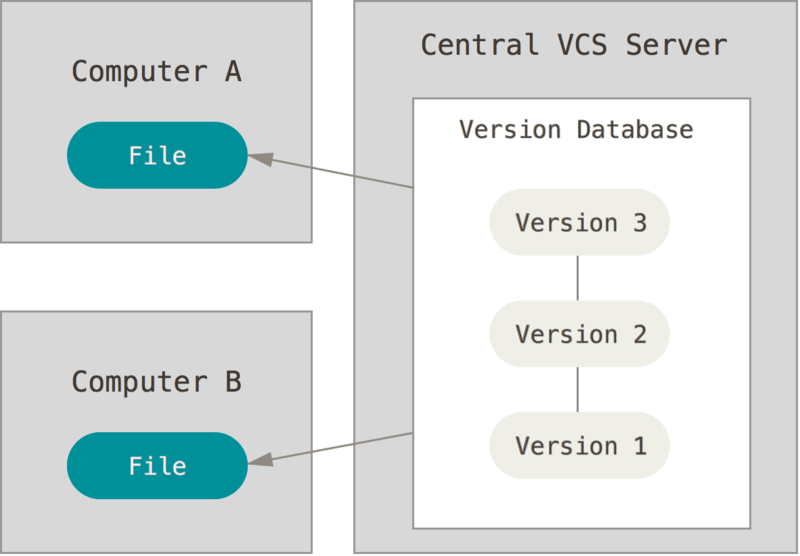
\includegraphics[scale=0.25]{Gambar/centralizedvcs.png}
	\caption{Centralized version control}
	\label{fig:cvcs}
\end{figure}

\textit{Local Version Control} hanya menyimpan \textit{file} pada satu komputer saja. Muncul masalah baru ketika \textit{user} ingin berkolaborasi dengan \textit{user} lain. Untuk mengatasi masalah ini dikembangkan \textit{Centralized version control}. Gambar \ref{fig:cvcs} merupakan struktur dari \textit{Centralized Version Control Systems}. Dalam \textit{Centralized Control Version Systems} terdapat sebuah \textit{server} yang menyimpan setiap versi \textit{file}, dan klien yang dapat melakukan \textit{checkout} \textit{file}\cite{chacon2014pro}.

Sistem \textit{Centralized Version Control Systems} memiliki beberapa kelebihan. Setiap \textit{user}  dapat mengetahui pekerjaan yang dilakukan oleh \textit{user} lain. Administrator dapat lebih mudah mengontrol \textit{database} \textit{Centralized Version Control Systems} dibandingkan dengan \textit{database} \textit{Local Version Control Systems} dari setiap klien.      

Tetapi, \textit{Centralized Version Control Systems} juga memiliki kelemahan. Jika \textit{server} pusat \textit{Centralized Version Control Systems} mati , maka perubahan pada \textit{file} tidak bisa disimpan. Klien juga tidak dapat melakukan kolaborasi dengan klien lain. Jika \textit{harddisk} pada server rusak, maka semua versi \textit{file} akan hilang.  

\subsubsection{Distributed Version Control Systems}
\begin{figure}[H]
	\centering
		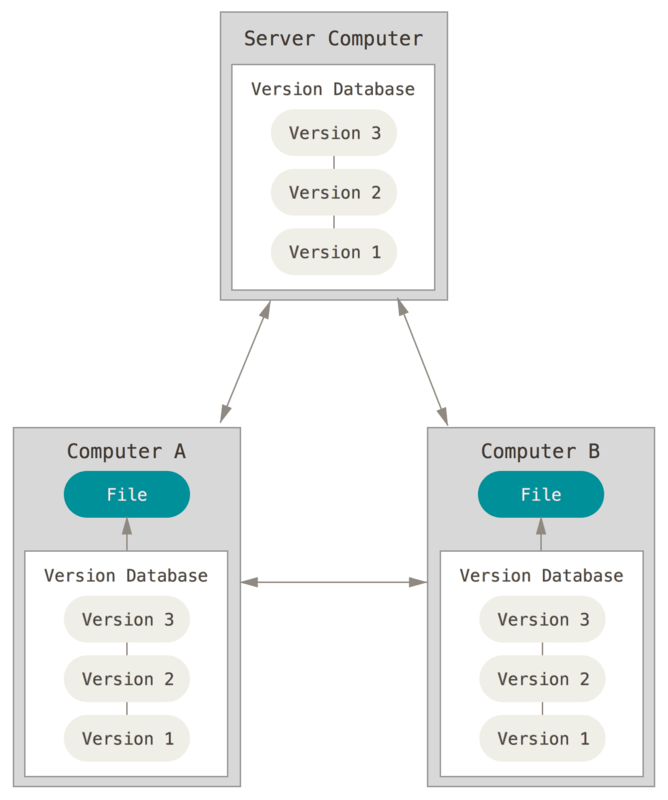
\includegraphics[scale=0.5]{Gambar/dvcs.png}
	\caption{Distributed version control}
	\label{fig:dvcs}
\end{figure}
Gambar \ref{fig:dvcs} merupakan struktur dari \textit{Distributed Version Control Systems}. Dalam sebuah DVCS (seperti Git, Mercurial, Bazaar atau Darcs), klien tidak hanya melakukan \textit{checkout} untuk \textit{snapshot} terakhir setiap \textit{file}, namun klien juga memiliki salinan dari repositori tersebut\cite{chacon2014pro}. Dengan kata lain setiap klien memiliki \textit{version database local} pada komputernya. Jika server pusat mati, klien masih bisa melakukan kolaborasi dan klien manapun dapat mengirimkan kembali salinan repositori ke \textit{server}.

\subsection{Cara Kerja Git}
\label{subsec:cara_kerja_git}
Salah satu perbedaan antara Git dengan VCS lainnya adalah dalam cara Git memperlakukan datanya\cite{chacon2014pro}. Kebanyakan sistem \textit{Version Control Systems} lain menyimpan informasi sebagai daftar perubahan \textit{file}. Pada Gambar \ref{fig:deltas}, terdapat tiga \textit{file}.\textit{Version Control Systems} menyimpan \textit{file} A, B, dan C pada versi pertama saja. Untuk versi kedua dan seterusnya yang disimpan adalah perubahan pada setiap \textit{file}. Sistem ini disebut juga sebagai \textit{delta-based Version Control Systems}. 
\begin{figure}[H]
	\centering
		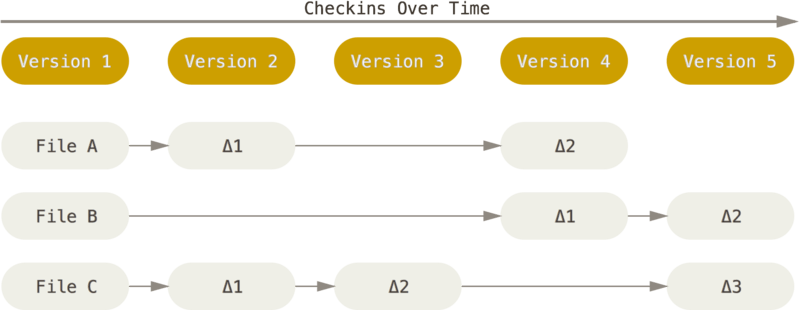
\includegraphics[scale=0.5]{Gambar/deltas.png}
	\caption{Menyimpan data sebagai \textit{snapshots} dari \textit{project}}
	\label{fig:deltas}
\end{figure}


Berbeda dengan \textit{Version Control Systems} lainnya, Git memperlakukan datanya sebagai sebuah kumpulan \textit{snapshot} dari sebuah miniatur \textit{file system}\cite{chacon2014pro}. Setiap kali dilakukan \textit{commit}, git merekam \textit{state} dari sekumpulan \textit{file} dan menyimpanannya sebagai \textit{reference} \textit{snapshot} tersebut. Gambar \ref{fig:snapshots}, menunjukkan \textit{snapshots} dari \textit{file} A, B, dan C. Pada versi kedua, \textit{file} B tidak mengalami perubahan, sehingga \textit{file} yang disimpan adalah referensi \textit{file} B pada versi sebelumnya.
\begin{figure}[H]
	\centering
		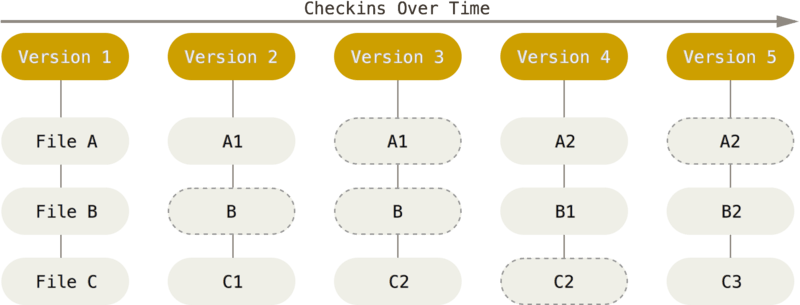
\includegraphics[scale=0.5]{Gambar/snapshots.png}
	\caption{Menyimpan data sebagai perubahan terhadap versi dasar dari setiap \textit{file}}
	\label{fig:snapshots}
\end{figure}

\subsubsection{State pada Git}
Terdapat tiga \textit{state} pada Git yaitu \textit{committed}, \textit{modified}, and \textit{staged}\cite{chacon2014pro}.\textit{Committed} adalah \textit{state} dimana data sudah disimpan di \textit{local database}. \textit{Modified} \textit{state} dimana terdapat perubahan pada \textit{file}, namun \textit{file} tersebut belum di \textit{commit} ke \textit{database}. \textit{Staged} adalah \textit{state} dimana \textit{file} telah ditandai untuk kemudian dilakukan commit.

Terdapat tiga bagian utama dari sebuah \textit{project} Git yaitu direktori Git, direktori kerja, dan staging area\cite{chacon2014pro}. Direktori Git merupakan tempat dimana Git menyimpan \textit{metadata} dan \textit{object database} dari \textit{project}. \textit{Working ree} adalah suatu \textit{snapshot} dari \textit{project}. Sekumpulan \textit{file} ini diambil dari \textit{database} di direktori Git dan ditempatkan pada \textit{disk} untuk digunakan dan dimodifikasi. \textit{Staging} area adalah \textit{file} yang menyimpan informasi mengenai apa yang menjadi \textit{commit} selanjutnya. \textit{File staging area} terdapat pada direktori Git. Untuk lebih jelasnya, lihat Gambar \ref{fig:git_state}.

Alur kerja dari Git adalah sebagai berikut:
\begin{enumerate}
\item Melakukan modifikasi pada \textit{file}
\item Menandai perubahan pada \textit{file} dan memindahkannya ke \textit{staging area}.
\item Mengambil \textit{file} dari \textit{staging area} dan menyimpan \textit{snapshot} ke direktori Git. Proses ini disebut dengan \textit{commit}.
\end{enumerate}  

\begin{figure}[H]
	\centering
		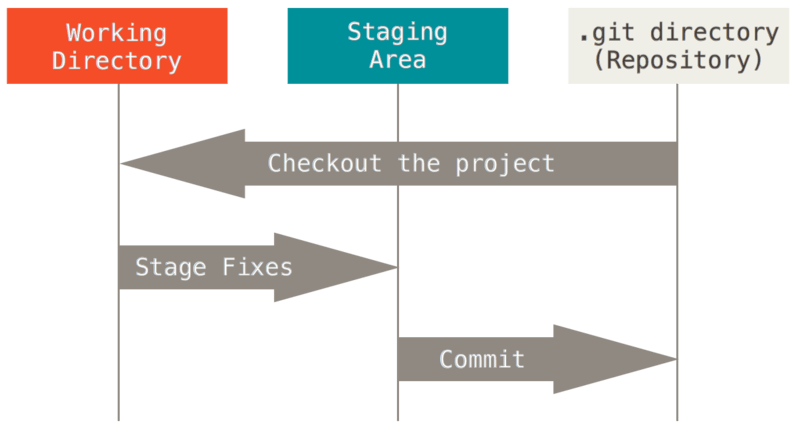
\includegraphics[scale=0.5]{Gambar/git_state.png}
	\caption{ \textit{Working tree}, \textit{Staging area}, dan Git direktori}
	\label{fig:git_state}
\end{figure}

\subsubsection{Commit}
Commit merupakan sebuah \textit{snapshot} dari suatu \textit{file} atau direktori. \textit{Commit} menggambarkan \textit{state} dari \textit{working directory}. Gambar \ref{fig:snapshots} menunjukkan terdapat tiga \textit{file} pada versi/\textit{commit} keempat. Dimana terdapat \textit{file} A1, B1, dan C1 pada \textit{working directory}. \textit{File} A1, B1, dan C2  merupakan \textit{state} \textit{file} A, B, dan C pada \textit{commit} keempat. 

Git melakukan \textit{check-summed} pada \textit{commit} sebelum menyimpannya ke Git repositori. Mekanisme yang digunakan untuk melakukan \textit{check-summed} disebut dengan \textit{SHA-1 hash}\cite{chacon2014pro}. \textit{SHA-1 hash} terdiri dari empat puluh karakter heksadesimal(0-9 a-f). Nilai dari \textit{SHA-1 hash} dihitung berdasarkan isi dari \textit{working directory} atau struktur direktori Git.

\begin{figure}[H]
	\centering
		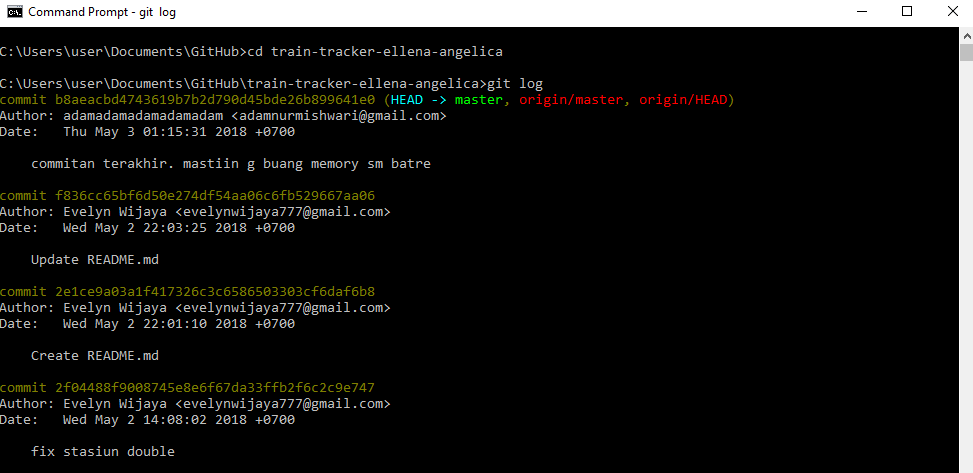
\includegraphics[scale=0.6]{Gambar/contoh_commit_history.png}
	\caption{Contoh histori \textit{commit} dalam pengembangan perangkat lunak}
	\label{fig:git_histori}
\end{figure}

Seperti yang diperlihatkan pada Gambar \ref{fig:git_histori}, setiap \textit{commit} memiliki beberapa informasi. Baris pertama menunjukkan \textit{commit} ID yang berupa \textit{SHA-1 hash}. Pada baris ini, \textit{Master} menunjukkan \textit{branch} yang sedang aktif, \textit{master} juga merupakan \textit{pointer} ke \textit{commit} terakhir. \textit{Head} merupakan \textit{reference} ke \textit{branch master}. \textit{Origin}/\textit{master} dan \textit{origin}/\textit{HEAD} merupakan \textit{master} dan \textit{HEAD} pada \textit{remote repository}. Baris kedua menunjukkan orang yang melakukan \textit{commit} dan alamat emailnya. Baris ketiga menunjukkan waktu terjadinya \textit{commit}. Baris terakhir berisi deskripsi dari \textit{commit} tersebut.

\subsection{Operasi Dasar pada Git}
\label{subsec:operasi_dasar_git}
Pada subbab ini dijelaskan mengenai operasi dasar dalam Git dan sintaks-sintaksnya. Sintaks-sintaksnya ini dimasukkan pada Git \textit{command line}. Berikut ini adalah operasi-operasi dasar dalam Git:
\begin{enumerate}
\item Init\\
Operasi ini digunakan untuk membuat repositori lokal baru dengan nama tertentu. Bisa juga digunakan untuk merekam direktori yang sudah ada. Berikut adalah sintaks untuk melakukan operasi  \textit{init}:\\
\$ git init [project-name]
\item Add\\
Operasi ini digunakan untuk menandai perubahan pada \textit{file} dan memindahkan \textit{file} tersebut ke \textit{staging area}. Operasi ini juga digunakan untuk menambahkan \textit{file} yang dipantau perubahannya. Berikut adalah sintaks untuk melakukan operasi add:\\
\$ git add [file]
\item Commit\\
Operasi digunakan untuk merekam \textit{snapshot} atau \textit{state} \textit{file} atau sekumpulan \textit{file}. Operasi ini juga digunakan untuk memindahkan \textit{file} yang berada di \textit{stagging area} ke repositori Git. Berikut adalah sintaks untuk melakukan operasi \textit{commit}:\\
\$ git commit -m "[descriptive message]"
\item Branch\\
Operasi ini digunakan untuk menampilkan semua \textit{branch} yang ada pada repositori Git, membuat \textit{branch} baru, dan menghapus \textit{branch}. Berikut adalah sintaks-sintaks untuk melakukan operasi \textit{branch}:\\
\$ git branch\\
\$ git branch [branch-name]\\
\$ git branch -d [branch-name]\\
\$ git branch -D [branch-name]
\item Diff\\
Operasi ini digunakan untuk menampilkan perbedaan pada \textit{file} yang belum masuk \textit{staging area}, menampilkan perbedaan pada \textit{file} yang berada di \textit{staging area} dengan \textit{file} di \textit{commit} sebelumnya, dan perbedaan \textit{file} antara dua \textit{branch}.  Berikut adalah sintaks-sintaks untuk melakukan operasi \textit{diff}:\\
\$ git diff \\
\$ git diff --staged\\
\$ git diff [first-branch]...[second-branch]
\item Clone\\
Operasi ini digunakan untuk menyalin repositori Git yang berada di komputer lain atau suatu \textit{server}. Berikut adalah sintaks untuk melakukan operasi \textit{clone}:\\
\$ git clone [url]
\item Fetch\\
Operasi ini digunakan untuk mengambil data dari \textit{remote} repositori ke repositori lokal. Berikut adalah sintaks untuk melakukan operasi \textit{fetch}:\\
\$ git fetch [bookmark]
\item Merge\\
Operasi ini digunakan untuk menggabungkan \textit{branch} tertentu dengan \textit{branch} yang sedang aktif. Operasi ini juga digunakan untuk menggabungkan data yang diambil dari \textit{remote} repositori dengan data pada \textit{working directory}. Berikut adalah sintaks untuk melakukan operasi \textit{merge}:\\
\$ git merge [branch]/[bookmark]
\item Pull\\
Operasi ini adalah gabungan dari operasi \textit{fetch} dan \textit{merge}. Berikut adalah sintaks untuk melakukan operasi \textit{pull}:\\
\$ git pull
\item Push\\
Operasi ini digunakan untuk mengirim data pada reposipori Git lokal ke \textit{remote repository}.
Berikut adalah sintaks untuk melakukan operasi \textit{push}:\\
\$ git push [alias] [branch]
\item Checkout\\
Operasi ini digunakan untuk berpindah ke \textit{branch} atau \textit{commit} tertentu, setelah itu memperbarui \textit{file} pada \textit{working directory} berdasarkan \textit{branch} atau \textit{commit} tersebut. Berikut ini adalah sintaks-sintaks untuk operasi \textit{checkout}:\\
\$ git checkout [SHA-1 commit]\\
\$ git checkout [branch-name]
\item Log\\
Operasi ini digunakan untuk menampilkan semua histori \textit{commit} pada \textit{branch} yang sedang aktif. Berikut ini adalah sintaks untuk melakukan operasi \textit{log}:\\
\$ git log
\end{enumerate}
\subsection{Git Checkout}
Seperti yang sudah dijelaskan pada subbab \ref{subsec:operasi_dasar_git}, \textit{checkout} dapat digunakan untuk berpindah ke \textit{branch} atau \textit{commit} tertentu. Operasi \textit{checkout} dapat dilakukan menggunakan sintaks "\$ git checkout" diikuti dengan nama \textit{branch} atau \textit{SHA-1 hash}. Gambar \ref{fig:git_checkout} menunjukkan contoh \textit{checkout} pada \textit{commit}. Posisi awal \textit{HEAD} menunjuk pada \textit{branch master}, setelah dilakukan \textit{checkout} ke \textit{commit kedua}, posisi \textit{HEAD} menunjuk pada \textit{commit kedua}. \textit{Working directory} diperbarui berdasarkan \textit{state} pada \textit{commit} kedua. 
\begin{figure}[H]
	\centering
		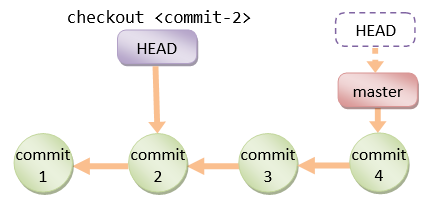
\includegraphics[scale=0.7]{Gambar/gitcheckoutcommit.png}
	\caption{\textit{Checkout} pada \textit{commit}}
	\label{fig:git_checkout}
\end{figure}

\section{JGit}
\label{sec:jgit}
JGit adalah \textit{library} Java murni yang mengimplementasikan Git \textit{version control systems}\cite{JGit}. Dengan menggunakan JGit, operasi-operasi dalam Git bisa dilakukan melalui program Java. Pada subbab berikut dijelaskan beberapa kelas dari \textit{library} JGit. 

\subsection{Repository}
\label{subsec:repository}
Kelas ini merepresentasikan repositori Git\cite{JGit_java_doc}. Berikut ini adalah beberapa \textit{method} dalam kelas ini:
\begin{itemize}
\item public void create() throws IOException\\
Berfungsi untuk membuat repositori Git baru.
\item public void create(boolean bare) throws IOException\\
Berfungsi untuk membuat repositori Git baru. \\
Parameter: jika bernilai \textit{true} maka dibuat \textit{bare repository} (repositori tanpa \textit{working directory}). 
\end{itemize} 

\subsection{Git}
\label{subsec:Git}
Kelas ini menyediakan API yang mirip GitPorcelain untuk berinteraksi dengan repositori git\cite{JGit_java_doc}. Berikut ini adalah beberapa \textit{method} dalam kelas ini:
\begin{itemize}
\item public LogCommand log()\\
\textit{Method} ini mengembalikan objek \textit{command} untuk mengeksekusi operasi \textit{Log}.\\
Kembalian: objek \textit{LogCommand} yang berfungsi untuk mengumpulkan parameter opsional dan akhirnya mengeksekusi operasi \textit{Log}.
\item public CheckoutCommand checkout()\\
\textit{Method} ini mengembalikan objek \textit{command} untuk mengeksekusi operasi \textit{checkout}.\\
Kembalian: objek \textit{CheckoutCommand} yang berfungsi untuk mengumpulkan parameter opsional dan akhirnya mengeksekusi operasi \textit{checkout}.
\item public CommitCommand commit()\\
\textit{Method} ini mengembalikan objek \textit{command} untuk mengeksekusi operasi \textit{commit}.\\
Kembalian: objek \textit{CommitCommand} yang berfungsi untuk mengumpulkan parameter opsional dan akhirnya mengeksekusi operasi \textit{commit}.
\end{itemize}

\subsection{RevWalk}
\label{subsec:revwalk}
Kelas ini digunakan untuk menelusuri \textit{commit graph}.  Berikut ini adalah beberapa \textit{method} dalam kelas ini:
\begin{itemize}
\item public RevCommit parseCommit(AnyObjectId id)\\
Menempatkan \textit{reference} ke suatu \textit{commit} kemudian melakukan \textit{parsing} pada isi \textit{commit}.
Parameter: nama dari objek \textit{commit}.\\
Kembalian: \textit{reference} ke objek \textit{commit}.
\item public void sort(RevSort s)\\
Berfungsi untuk mengurutkan \textit{commit} berdasarkan metode dari parameter.\\
Parameter: metode untuk mengurutkan \textit{commit}.
\end{itemize}

\subsection{RevCommit}
\label{subsec:revcommit}
Kelas ini merupakan \textit{reference} ke \textit{commit} yang ada di \textit{Directed Acyclic Graph}\cite{JGit_java_doc}. Berikut ini adalah beberapa \textit{method} dari kelas ini:
\begin{itemize}
\item public final String getFullMessage()\\
Berfungsi untuk melakukan \textit{parsing} pada \textit{commit message} dan mengubahnya ke \textit{string}.\\
Kembalian: \textit{string} hasil \textit{decode} dari \textit{commit message}.
\item public final String getName()\\
\textit{Method} ini mengembalikan \textit{SHA-1} dalam bentuk \textit{string}.
\end{itemize}

\section{Selenium WebDriver}
\label{sec:selenium_webdriver}
Selenium adalah kumpulan dari kakas perangkat lunak, dengan pendekatan yang berbeda pada setiap kakas dalam mendukung \textit{automation test}\cite{Selenium_doc}. Selenium mendukung bahasa pemrograman C\#, Java, Perl, PHP, Python, Ruby, dan JavaScript. Selenium terdiri dari beberapa kakas, yaitu Selenium 1(Selenium RC), Selenium 2(Selenium WebDriver), Selenium-Grid, dan Selenium IDE. Selenium RC merupakan proyek utama \textit{Selenium} untuk waktu yang lama, sebelum akhirnya bergabung dengan \textit{WebDriver} menjadi Selenium 2. Selenium RC bekerja dengan cara menginjeksi kode JavaScript ke \textit{browser} ketika \textit{browser} dimuat dan menggunakan JavaScript tersebut untuk menggerakkan \textit{Application Under Test} dalam \textit{browser}. Selenium RC sekarang sudah \textit{deprecated}/tidak digunakan lagi. Selenium Webdriver merupakan gabungan dari Selenium RC dan WebDriver. Selenium IDE merupakan \textit{prototyping} kakas untuk membangun \textit{script test}.

WebDriver merupakan kakas untuk mengotomatisasi pengujian pada perangkat lunak web\cite{Selenium_doc}. WebDriver dapat berkomunikasi dengan \textit{browser} menggunakan \textit{native support} pada\textit{browser} untuk automasi. Setiap \textit{browser} memiliki WebDriver masing-masing. WebDriver yang terdapat pada SeleniumDriver antara lain ChromeDriver, FirefoxDriver/GeckoDriver, OperaDriver, InternetExplorerDriver, dan HtmlUnitDriver. 

Pada skripsi ini \textit{tools} Selenium yang digunakan hanya Selenium WebDriver. WebDriver yang digunakan adalah ChromeDriver. Bahasa yang digunakan adalah Java. Pada subbab berikut dijelaskan beberapa kelas dari \textit{library} Selenium WebDriver. 
\cite{Selenium_java_doc}
\subsection{WebDriver}
\label{subsec:webdriver}
Kelas ini merupakan \textit{interface} utama yang digunakan untuk pengujian, kelas ini merepresentasikan \textit{web browser} yang ideal \cite{Selenium_java_doc}. Berikut ini adalah beberapa \textit{method} dalam kelas ini:
\begin{itemize}
\item void close()\\
Berfungsi untuk menutup \textit{window} pada \textit{browser}, jika \textit{window} yang sekarang merupakan satu-satunya \textit{window} yang terbuka maka \textit{browser} akan ditutup.
\item void quit()\\
Berfungsi untuk menutup driver dan semua \textit{window} yang sedang terbuka.
\item void get(String url)\\
Berfungsi untuk memuat halaman \textit{web} pada \textit{window} saat ini. \textit{Method} ini mengirim \textit{HTPP GET Request} untuk memuat halaman, dan \textit{method} ini akan melakukan \textit{blocking} sampai halaman \textit{web} selesai dimuat.\\
Parameter: alamat \textit{url} untuk memuat halaman \textit{web}.
\end{itemize}

\subsection{WebElement}
\label{subsec:webelement}  
Kelas ini adalah \textit{Interface} yang  merupakan representasi dari elemen HTML\cite{Selenium_java_doc}. Berikut ini adalah beberapa \textit{method} yang dimiliki kelas ini:
\begin{itemize}
\item void click()\\
Berfungsi untuk mengklik suatu elemen HTML.
\item void submit()\\
Berfungsi untuk mengirimkan elemen \textit{form} ke \textit{remote server}. Fungsi ini akan melempar \textit{NoSuchElementException} jika elemen yang dikirim tidak berada di dalam \textit{form}. 
\item String getText()\\
Berfungsi untuk mendapatkan teks pada suatu elemen.\\
Kembalian: Teks yang \textit{visible} pada elemen.

\item void clear()\\
Berfungsi untuk menghapus teks pada elemen yang digunakan untuk memasukkan teks.
\item WebElement findElement(By by)\\
Berfungsi untuk mendapatkan \textit{WebElement} pertama menggunakan metode yang diberikan parameter. \textit{Method} ini akan melempar \textit{NoSuchElementException} jika \textit{WebElement} tidak ditemukan.\\
Kembalian: \textit{WebElement} pertama yang sesuai dengan mekanisme pencarian.\\
Parameter: mekanisme pencarian, bisa berupa pencarian dengan \textit{ID}, \textit{class}, dll.

\item List<WebElement> findElements(By by)\\
Berfungsi untuk mendapatkan semua \textit{WebElement} sesuai dengan mekanisme yang diberikan parameter.\\
Kembalian: \textit{list} dari \textit{WebElement}, atau \textit{list} kosong jika pencarian tidak ditemukan.\\
Parameter: mekanisme pencarian, bisa berupa pencarian dengan \textit{ID}, \textit{class}, dll.
\item void sendKeys(java.lang.CharSequence... keysToSend)\\
Berfungsi untuk mengirimkan kumpulan karakter/teks ke elemen \textit{input}. \textit{Method} ini akan melempar \textit{java.lang.IllegalArgumentException} jika parameter keysToSend bernilai \textit{null}.\\
Parameter: kumpulan karakter/teks yang dikirim ke elemen.
\end{itemize} 

\subsection{OutputType}
\label{subsec:output_type}
Kelas ini merupakan \textit{interface} yang menentukan tipe \textit{output} pada \textit{screenshot}\cite{Selenium_java_doc}. Terdapat tiga konstanta untuk menentukan tipe \textit{output} pada \textit{screenshot}. Konstanta tersebut adalah sebagai berikut:
\begin{itemize}
\item static final OutputType<String> BASE64]\\
Berfungsi untuk mendapatkan \textit{screenshot} dalam bentuk \textit{base64 data}.
\item static final OutputType<byte[]> BYTES\\
Berfungsi untuk mendapatkan \textit{screenshot} dalam bentuk \textit{raw bytes}.
\item static final OutputType<java.io.File> FILE\\
Berfungsi untuk mendapatkan \textit{screenshot} dalam bentuk \textit{temprorary file} yang akan dihapus setelah program keluar dari \textit{Java Virtual Machine}.
\end{itemize}


\subsection{TakesScreenshot}
\label{subsec:takes_screenshot}
Kelas ini merupakan \textit{interface} yang digunakan untuk mengambil \textit{screenshot}. Kelas ini hanya mempunyai satu method yaitu:
\begin{itemize}
\item <X> X getScreenshotAs(OutputType<X> target) throws WebDriverException\\
\textit{Method} ini berfungsi untuk mengambil \textit{screenshot} dan menyimpannya ke lokasi yang sudah ditentukan. Kelas\\
Kembalian: objek yang menyimpan informasi terkait \textit{screenshot} \\
Parameter: tipe \textit{output} yang diinginkan(lihat \ref{subsec:output_type}).

\end{itemize}


\section{Apache Commons CLI}
\label{subsec:apache_cli}
